\documentclass[letterpaper,11pt]{article}

% So we can change the margins
\usepackage{geometry}

% This is needed for the includegraphics command.
\usepackage{graphicx}

% For the pretty bibliography
\usepackage{natbib}

% For fancy PDF hyperlinks and metadata
\usepackage[
  pdfauthor={MIDN 1/C Matthew J.P. Yates},
  pdftitle={Computing with sparse integers},
  colorlinks,linkcolor=black,urlcolor=black,citecolor=black
]{hyperref}

% For typesetting algorithms
\usepackage[ruled,vlined]{algorithm2e}
\DontPrintSemicolon

\begin{document}

\title{Computing with sparse integers}

\author{MIDN 1/C Matthew J.P.~Yates\\[2mm]
{\small Advisor: Asst.~Prof.~Daniel S.~Roche}\\
{\small Computer Science Department}\\
{\small United States Naval Academy}
}

\date{\today}

\maketitle

\begin{abstract}
  We explore some
  algorithmic aspects of arithmetic with \emph{sparse integers}. 
  numbers in which only the nonzero bits are explicitly represented. 
  The \emph{sparse signed digit} representation is proposed as a good
  balance between expressiveness and speed, and under this representation
  we present algorithms for basic arithmetic including multiplication,
  division with remainder, and modular exponentiation. Finally, a 
  high-performance
  C library implementation of these routines is examined and compared
  to existing approaches.
\end{abstract}

\section{Introduction} 
Traditionaly Intergers are held with an array of bits. At each position $n$ in the array the bit, ethier a $0$ or $1$, 
acts a coeffient for $2^{n}$. This is repeated for every position to convert to the base 10 version of the number.
This approch has a limitation in how large of an number can be stored. The 32 bit unsigned integer can represent up to $8589934591$
before every combination of 0's and 1's for each of the 32 bits has been used. This maximum may be large enougth for many applications, but 
in certain feilds, such as Cryptography increbly large integers that exceed normal 32, 64, or even 128 bit integers are required.
In these instances not even a largest primitive types can be trusted to not
overflow in the process of computing an answer. The solution to this is
to use non primitive numbers data types for integers, such as a BigInt.
A BigInt stores arbitrarily large numbers using an ever expanding buffer to hold the bits of any
number for which the computer has enough disk space to hold. 
One shortcoming with the BigInt approach is that they hold every single bit, even
if the number may have 99\% of its bits as 0's. This sort of number is
considered to be sparse.  The sparse number may be held more efficiently
if only the locations of where the set bits exist. 
Sparse Integers are a way of holding certain incredibly large numbers in relatively 
little memory space when compared to traditional implementations.
With this conversion memory space need for huge numbers can greatly reduced, and in for some
mathematical operations, the Sparse Representation is faster than the traditional storage methods.

(Elaborate more here.) Various algorithms for
long integer arithmetic are covered
extensively in \cite{BZ10}. The sparse signed digit representation
is based on the non-adjacent form (NAF) first presented by
\cite{Rei60}. \cite{vui09} recently looked at a completely different
way of representing sparse integers.
Sparse integers have been studied in the context
of cryptography by \cite{bs02}, and are specified in standards such
as \cite{nis09}.

\section{Signed digit representation}
The signed representation works
with a series of signs, differences between positions, and size of the
highest set bit. 

For exapmle concider the following base 10 number $34359738240$
\begin{enumerate}
    \item base 10 $34359738240$
	\item base 2 $11111111111111111111111111110000000$
    \item base 2 signed ++++++++++++++++++++++++++++0000000
    \item base 2 after canceling +0000000000000000000000000000-000000
    \item sparse signed positions $+35 -7$
    \item sparse signed difference $+28 -7$
	\item with the top position $+28 -7, 35$ 
\end{enumerate}
$34359738240$ would need to be represented with at least 5 bytes if held in traditional form, for it could
not be allocated a partial byte.
Where as in in singed sparse from it needs at only the two signed differences, and the highest position.
These can be held with three C chars and and two C bools. Which with a vector to hold the bools both could
be represented in one char. In total the sparse representation would take take 4 bytes to represent the number 
$34359738240$. The space savings are amplified as the size of the number increases.
\section{Arithmetic} 
In addition to the obvious savings in terms of
space complexity by only storing a few bytes to reprsent numbers that could require kilobytes or more for 
a traditional bigint represetanation, some arthmetic operations will be faster than the bigInt equilvelent.

\subsection{Rules for Operands}
Whenever numbers are passed to signed sparse arithmetic operations, 
our model assumes that lists of bits are ordered by size and that they are the sparsest possible
representations of their numbers with no repeated bits. The modle also assumes that every bit is given a sign.


\subsection{Carry Logic} The advantage of signed bits is that negative
bits allow for many more numbers to represented in a sparse form and
that many small operations will not case a sudden increase in density of
the number.  The heuristic for sparsity is that the most sparse
representation of any number will have no two consecutive set bits.  

Two same signed bits at the same position will lead to a new bit being
placed one position higher with the same sign as the two matching bits.
The two matching bits will be removed. Two bits with matching positions
but not matching signs will be both removed.  If one bit is one position
lower than the other and they share signs then the lower bit will have
its sign flipped and the higher bit will have its position incremented
by one.  If two bits are one apart in position and are different signs
then the higher placed bit is removed and the lower bit has its sign
flipped.
\begin{algorithm}[Htbp]
  \caption{The carry Algorithm}
  \KwIn{Sparse Int $a$ and new set position $n$ such that $n >= a[-1]$}
  \KwOut{Sparse integer $b$ that is $a$ with the new position appended}
	$b \gets a$ \;
	  \If{$b[-1] = n$}{
	   \eIf{Signs of $a[-1]$ and $n$ are the same}{
		   $a[-1] \gets a[-1] + 1$\;
	   }{
		   popback($a$)\;
	   }
	return\;
    }
     \If{$b[-1] + 1 = n$}{
       \eIf{Signs of $a[-1]$ and $n$ are the same}{
           $a[-1] \gets a[-1] * - 1$\; flip the sign of the last element
		   pushback($a$,$n+1$)\; add the new position + 1
       }{
           $a[-1] \gets a[-1] * - 1$\; flip the sign of the last element and do not add a new bit
       }   
    return\;
    }
	pushback($a$,$n$)\; if the other steps did not return than there is no carry and the new position is just added

\end{algorithm}


\subsection{Addition and subtraction} Addition and subtraction are
 fundamentally achieved by combining two lists of signed bits by a merge
sort.  As the lists are combined the carry logic is applied for each bit
leaving the result in its most sparse and in sorted order.  The
difference between subtraction and addition is that the subtraction has
the sign of each bit flipped before combining the two lists.

\begin{algorithm}[Htbp]
  \caption{Addition Algorithm}
  \KwIn{Two sparse integers $a$ and $b$}
  \KwOut{Sparse integer $c$ that is equal to $a + b$}
  $i, j \gets 0$ \;
  \While{$i < \#a$ and $j < \#b$}{
    \If{$a[i] < b[j]$}{
      $c \gets c + a[i]$ with Carry Logic \;
      $i \gets i + 1$
    }
    \If{$a[i] > b[j]$}{
      $c \gets c + b[j]$ with Carry Logic \;
      $j \gets j + 1$
    }
    \If{$a[i] = b[j]$}{
      \If{Signs of $a[i]$ and $b[i]$ are the same}{
        $c \gets c + 2a[i]$ with Carry Logic\;
      }
      $i \gets i + 1$ \;
      $j \gets j + 1$
    }
  }
\end{algorithm}

\subsection{Multiplication} 
Multiplication is solved by a summation of
the smaller of the two numbers with each iteration having been shifted
to the left  by a signed bit of the larger number.
\begin{algorithm}[Htbp]
  \caption{Multiplication Algorithm}
  \KwIn{Two sparse integers $a$ and $b$}
  \KwOut{Sparse integer $c$ that is equal to $a * b$}
  \eIf{$\#a > \#b$}{
   $long \gets a$\;
   $short \gets b$\;
   }{
   $long \gets a$\;
   $short \gets b$\;
   }
  $i, j, c \gets 0$ \;

  \While{$i < \#long$}{
	  $c \gets c + short << long[i]$ \;
	$i \gets i +1$
    }
  }
\end{algorithm}


\subsection{Division with remainder} Division is essentially solved
through repeated subtraction of two sparse numbers.  At each iteration
of subtraction the divisor is multiplied by the difference between the
difference between the position highest bit of the numerator and the the
position of the highest bit in the divisor.
\begin{algorithm}[Htbp]
  \caption{Division Algorithm}
  \KwIn{Two positive sparse integers $a$ and $b$}
  \KwOut{Sparse integer $c$ that is equal to $a / b$}
  $i, j, c \gets 0$ \;
	$numerator \gets a$
  \While{$numerator > b$}{
	  $c \gets c + numerator[-1] - b[-1]$
	  $numerator \gets numerator - b<<(numerator[-1] - b[-1])$ \;
    }
	\If{$numerator != 0$}
	{
		$c \gets c -1$
	}

  }
\end{algorithm}
Then the modulo operation is esentially division without any concern with how many times
the denominator was subtracted from the numerator.
\begin{algorithm}[Htbp]
  \caption{Modulo Algorithm}
  \KwIn{Two positive sparse integers $a$ and $b$}
  \KwOut{Sparse integer $c$ that is equal to $a \% b$}
  $i, \gets 0$ \;
    $c \gets a$
  \While{$numerator > b$}{
      $c \gets c - b<<(c[-1] - b[-1])$ \;
    }
  } 
\end{algorithm}


\subsection{Modular exponentiation} Modular exponentiation follow the
classic algorithm with the variation of having to perform logical checks
during the iteration to convert the number to positive signed only. 
\begin{algorithm}[Htbp]
  \caption{Modular Exponation Algorithm}
  \KwIn{Three sparse integers $a$, $b$, and $c$}
  \KwOut{Sparse integer $d$ that is equal to $a^{b} \% c$}
  $i, j \gets 0$ \;
  $d \gets 1$\;
  $base \gets b$
  $seenNegative \gets false$
  \While{$i < \#b$}{
	  $k \gets 0$
	  \While{$k < b[i]-j$}
	  {
		  $base \gets base * base \% c$
		  $k \gets k + 1$
		  \If{$seenNegative$}
		  {
			  $d \gets d * base \% c$
		  }
	  }
	  \If{$\!seenNegative$}
          {
              $d \gets d * base \% c$
          }
	  $seenNegative \gets ! signOf(b[i])$
	$i \gets i +1$
    }
  
\end{algorithm}

\section{Implementation} The Spares Int data structure is made using
C++ class with two template arguments.  The template argument S is used
for setting the data structure used to hold the difference between two
positions. The other template Argument is T for the data type used to
hold the position of the highest set bit. The differences between
positions and the signs of each position are held in a vector from STL.
The signs are held as bools for a vector of bools provides a signifigant
space savings. 

\section{Time Trails} Tests where run on how many times basic
mathmatical operations where run per second.  The horizontal axis
represents how large the highest set bit is in the traitional binary
represenation of the number; a sample was drawn from every 1000.  The
vertical axis represents how many bits where in the number; a sample was
drawn every 5.  Each point in the each plot had three randomly generated
pairs of operands that meet the highest bit and number of bits
requirements. Addition, Subtraction, Multiplaction, and explonential
modulus all use operands with equal input pramaters. Divison and Modulus
give the denominator half the number of set bits as the numerator.  The
green represents areas where Sparse Ints were able to perform more
operations per second.  The red show areas where GMP was able to do
more.
The exponential modulus graph made with same paramters as the graphs above, save that both axis 
represent sampling at every 50.


% Change margins so two images fit per page
\newgeometry{textheight=9in}

\begin{figure}  
\begin{center}  
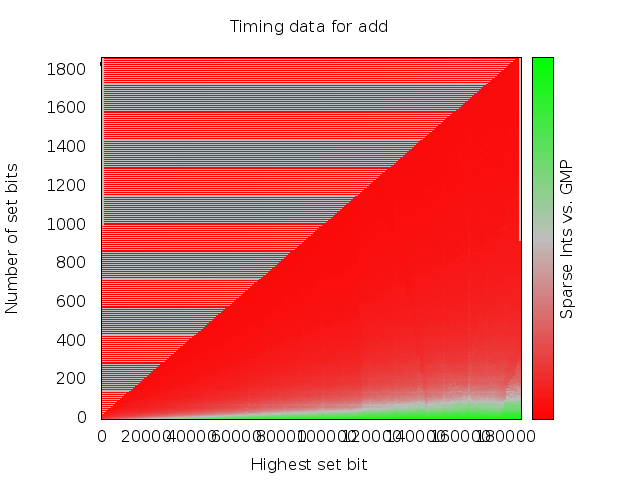
\includegraphics[width=.8\textwidth]{../plots/add5num1000high3test.png}  
\caption{\small \sl Sparse Int addition compared to GMP Addition\label{fig:Addition}}  
\end{center}  
\end{figure} 

\begin{figure}  
\begin{center}  
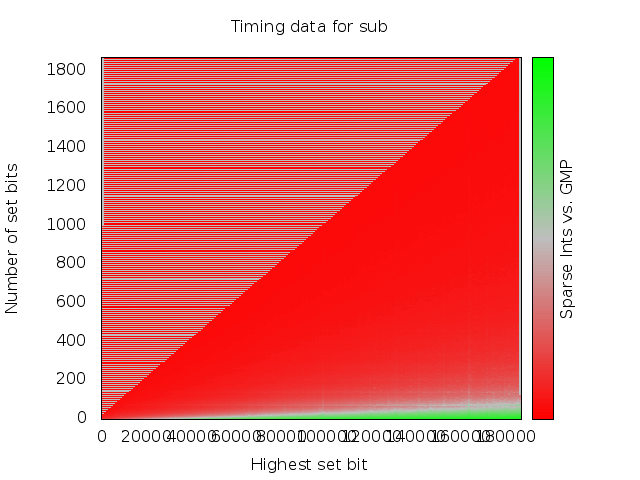
\includegraphics[width=.8\textwidth]{../plots/sub5num1000high3test.png}  
\caption{\small \sl Sparse Int subtraction compared to GMP subtraction\label{fig:Subtraction}}  
\end{center}  
\end{figure} 

\begin{figure}  
\begin{center}  
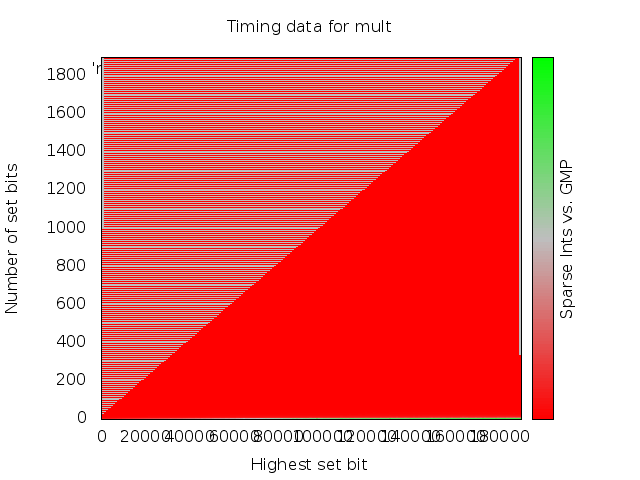
\includegraphics[width=.8\textwidth]{../plots/mult5num1000high3test.png}  
\caption{\small \sl Sparse Int multiplation compared to GMP multiplaction\label{fig:Multiplaction}}  
\end{center}  
\end{figure} 

\begin{figure}  
\begin{center}  
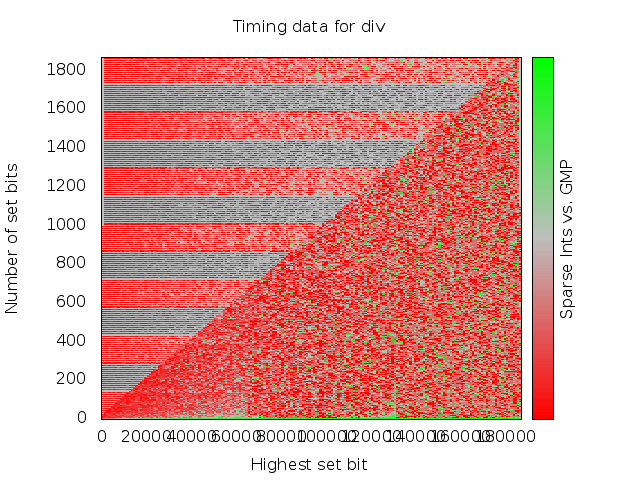
\includegraphics[width=.8\textwidth]{../plots/div5num1000high3test.png}  
\caption{\small \sl Sparse Int division compared to GMP division\label{fig:Division}}  
\end{center}  
\end{figure} 

\begin{figure}  
\begin{center}  
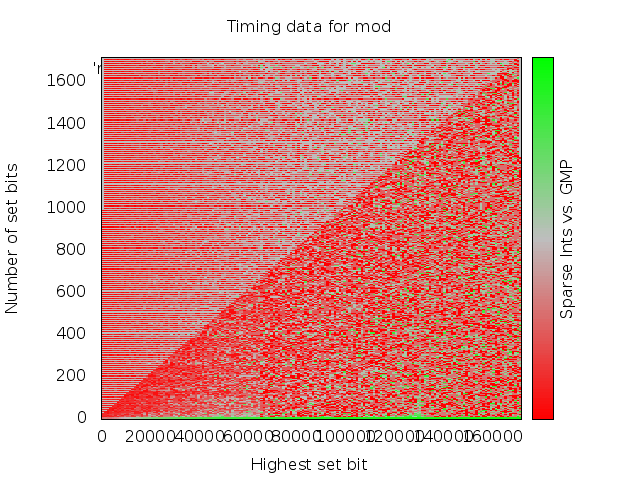
\includegraphics[width=.8\textwidth]{../plots/mod5num1000high3test.png}  
\caption{\small \sl Sparse Int modulus compared to GMP modulus\label{fig:Modulo}}  
\end{center}  
\end{figure} 

\begin{figure}  
\begin{center}  
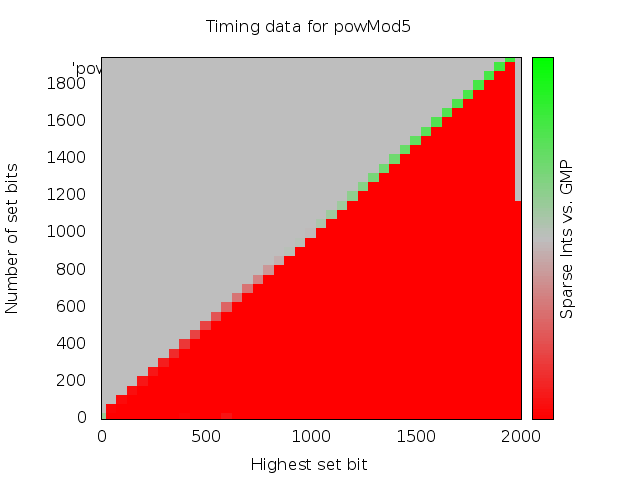
\includegraphics[width=.8\textwidth]{../plots/powMod50num50high3test.png}  
\caption{\small \sl Sparse Ints compared to GMP with regard to exponental moduls\label{fig:PowMod}}  
\end{center}  
\end{figure} 

% Undo margin changes
\restoregeometry

\section{Conclusion}
It is apperant that the GMP implementation for now is faster for a large varitey of cases. 
However it is important to note that in any case that is a tie, the gray colored areas, that Sparse Ints are 
using far less space to represent the same number. Using less space would mean more space in main memory may be saved for other aspects of
computation. 
\section{Future Work}
\begin{itemize}
    \item Work on decreasing the time complexity of the algorithms
    \item Expreriment with using thread is the number as large enough gaps in positions.
    \item Experiment with using a heap in multiplication to hold the result as it builds.
    \item Impliment an optimized squaring routine.
    \item Experiment with moving to a frequency domain as is used in polynomial multiplication.
\end{itemize}

% This is the references section.
\bibliographystyle{plainnat}
\bibliography{refs}

\end{document}
